\chapter{Hardware design of a low-cost sensor node}\label{chap3}

We use low-cost sensors we designed to detect on-off state change on each appliance, and to report to the single base station. The sensor plugs in an AC outlet, and provides one AC outlet for the appliance. Each appliance in question should connect to a separate sensor directly. Hence, an important design goal is low-cost. And we achieve the goal not by choosing cheap components, but simplifying the functionality. The extremely low price is inherent in the simplicity. 

%"Simplicity is the ultimate sophistication." - Leonardo Da Vinci

The functions and design goals of the sensor are
\begin{itemize}
  \item Detect binary (on-off) state changes
  \item Reliably deliver detected events to a central node
  \item Low cost
\end{itemize}

The overall block diagram of the sensor hardware is shown in Fig. \ref{fig:hwoverview}

%\begin{figure}[hb]
%  \centering
%  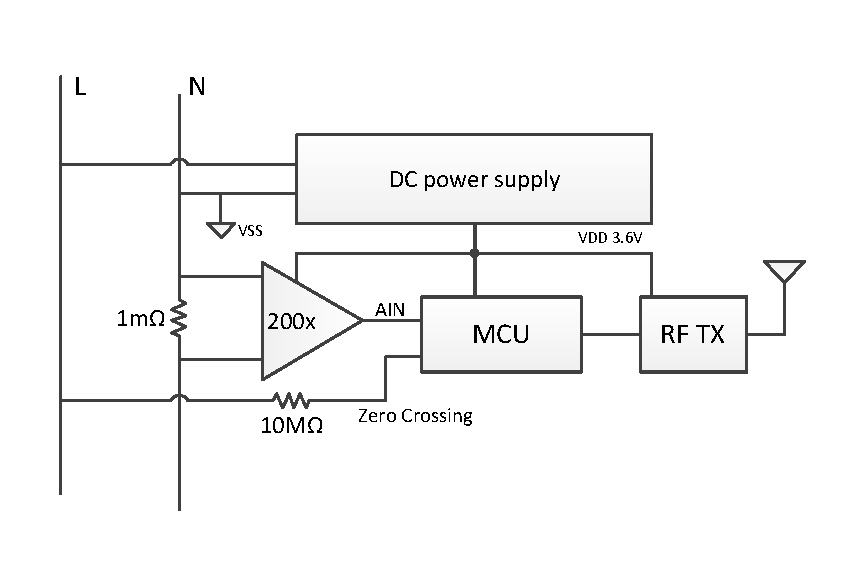
\includegraphics[width=0.5\textwidth]{fig/hwoverview}
%  \caption{Block diagram of the on-off state sensor hardware}
%  \label{fig:hwoverview}
%\end{figure}

\section{On-off state sensing}

As discussed before, one of the function of the sensor is to detect binary (on-off) state changes. This is achieved by processing the electrical current only, instead of the instantaneous power. Thus, voltage sampling is unnecessary, let alone the multiplier and adders. 
